  \subsection{Utilisation et implémentation}
  \begin{frame}
   \frametitle{Utilisation}

\begin{columns}
\begin{column}{7cm}
\begin{enumerate}[<+->]
    \item Choix du mode d'affichage Multi-Vues
    \item Séléction du nombre de vue
  	\item Choix de l'emplacement
  	\item Choix de la caméra
  	\item Visualisation de la caméra
  	\item Un clic long permet la visualisation et le controle de la caméra dans
  	la vue simple
\end{enumerate}
\end{column}
\begin{column}{6cm}
  \centering \includegraphics<1>[width=3cm]{Images/mvstep/s1.jpg}
  \centering \includegraphics<2>[width=3cm]{Images/mvstep/s2.jpg}
  \centering\includegraphics<3>[width=5cm]{Images/mvstep/s3.jpg}
  \centering \includegraphics<4>[width=5cm]{Images/mvstep/s4.jpg}
  \centering \includegraphics<5>[width=5cm]{Images/mvstep/s5.jpg}
  \centering \includegraphics<6>[width=5cm]{Images/mvstep/s6.jpg}
\end{column}
\end{columns}

  \end{frame}
 
  \begin{frame}
   \frametitle{Implémentation}
\centering 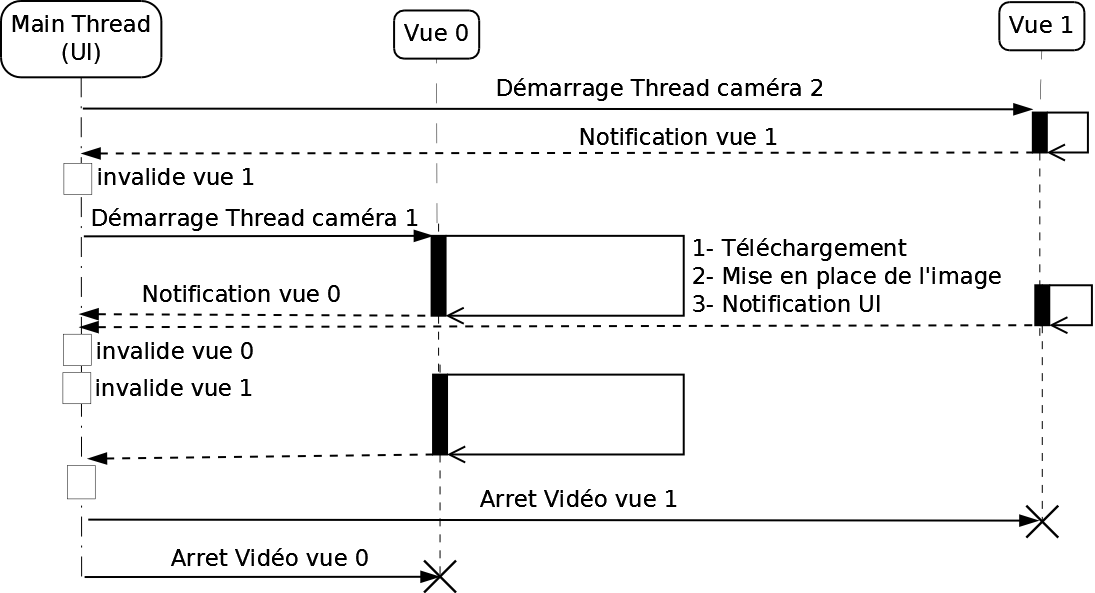
\includegraphics[scale=0.2]{Images/DiagrammeSequenceMultiView.png}

\begin{itemize}
    \item Chaques Threads notifient l'UI lorsqu'une nouvelle image est
    disponible
  	\item Delai réglable entre chaque début de téléchargement
  	\item Redessine uniquement la zone mise à jour
\end{itemize}
 \end{frame}
  